\chapter{Preliminary exploration of underwater IPT system}

% 为了探究实际情况中海水环境下的无线能量传输系统与空气中的无线能量传输系统的异同,这里使用了简单的双线圈结构对水下环境的电气属性进行了探究。本章将介绍双线圈结构在海水中工作的表现。
In order to explore the similarities and differences between the wireless energy transmission system in the seawater environment and the wireless energy transmission system in the air in the actual situation, a simple double-coil structure is used to explore the electrical properties of the underwater environment. This chapter will introduce the performance of the double coil structure working in sea water.




\section{Two ring coils WPT in the air}
In this chapter, our UWPT coil structure is as figure \ref{fig:3_two_ring_coil}.


\begin{figure}[htbp]
    \begin{subfigure}{0.5\textwidth}
        \centering
        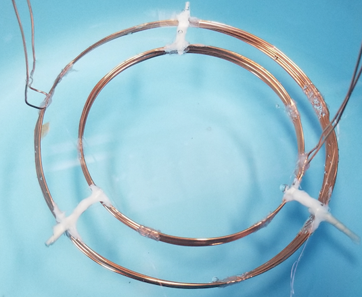
\includegraphics[width=0.9\linewidth]{images/3_two_ring_coil.png}
        \caption{Experimental coil.}
        \label{fig:subim1}
    \end{subfigure}
    \begin{subfigure}{0.5\textwidth}
        \centering
        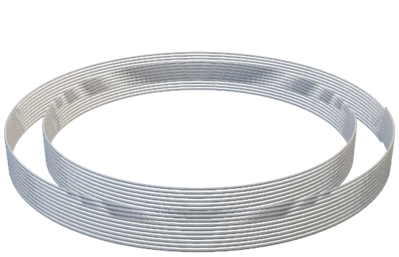
\includegraphics[width=0.9\linewidth]{images/3_two_ring_coil_structure.png}
        \caption{Structure diagram.}
        \label{fig:subim2}
    \end{subfigure}

    \caption{Two ring structure.}
    \label{fig:3_two_ring_coil}
\end{figure}

Its detailed parameters are shown in Table \ref{table:ring coil parameters}.

\begin{table}[htbp]
    \centering
    \caption{The parameters of ring coil structure.}
    \begin{tabular}{ c|cc }
        \thickhline
        % \hline
        \textbf{Items} & \textbf{Parameters}     \\
        \thickhline
        Environment    & Air, tap water, seawater \\ \hline
        Wire diameter  & 0.8mm                    \\ \hline
        Wire material  & Copper                   \\ \hline
        Turns          & 10                       \\ \hline
        Frequency      & 200kHz                   \\ \hline
    \end{tabular}
    \label{table:ring coil parameters}
\end{table}


\section{Two ring coils structure}
\subsection{Simulation evaluation}
\subsection{Experimental evaluation}

\section{Conclusion}

\begin{figure}[htbp]
    \centering
    
\includegraphics[width=0.4\linewidth]{images/3_mutual_inductance.png}
    \caption{Underwater sensor networks architecture.}
    \label{fig:3_mutual_inductance}
\end{figure}

\begin{figure}[htbp]
    \centering
    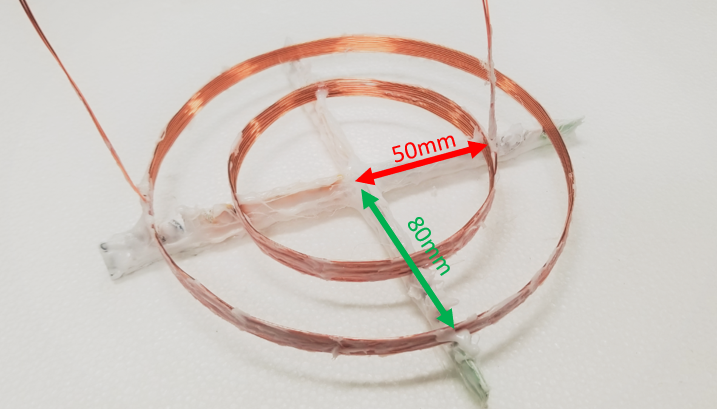
\includegraphics[width=0.7\linewidth]{images/3_two_ring_coil_5cm_8cm.png}
    \caption{Two ring structure ($Radius_{inner coil}=50mm$, $Radius_{outer coil}=80mm$).}
    \label{fig:3_two_ring_coil_5cm_8cm}
\end{figure}

\begin{figure}[htbp]
    \centering
    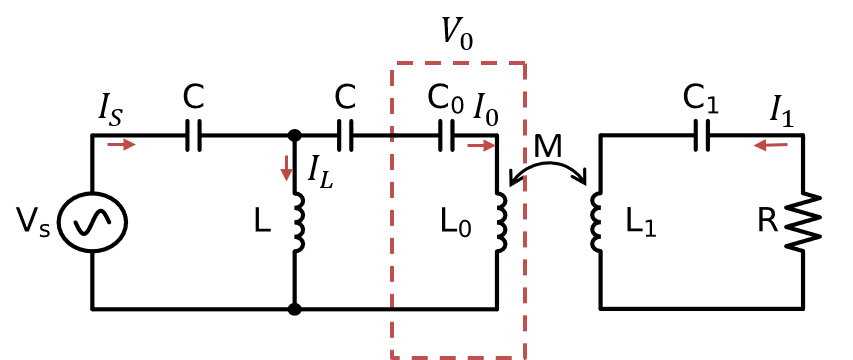
\includegraphics[width=0.8\linewidth]{images/3_clc_s_scheme.png}
    \caption{CLC-S Scheme.}
    \label{fig:3_clc_s_scheme}
\end{figure}